\documentclass[openany]{book}

\usepackage{amscd}
\usepackage{amsmath}
\usepackage{amssymb}
\usepackage{amsthm}
\usepackage{verbatim}
\usepackage[utf8]{inputenc}
\usepackage{geometry}
\geometry{letterpaper}
\usepackage[pdftex]{graphicx}
\usepackage{setspace}
\usepackage{physics}
\usepackage{subcaption}
\usepackage[numbers]{natbib}
\usepackage{pdfpages}
\usepackage{bm}
\usepackage{wrapfig}
\usepackage{color}
\usepackage{enumerate}
\usepackage{multicol}
\usepackage{float}
\usepackage{cancel}
\usepackage{hyperref}
\usepackage[dvipsnames]{xcolor}
\usepackage{nicefrac}
\usepackage[most]{tcolorbox}
\usepackage{listings}
\hypersetup{
    colorlinks=true,
    linkcolor=blue,
    filecolor=magenta,      
    urlcolor=cyan,
    pdftitle={Overleaf Example},
    pdfpagemode=FullScreen,
    }

\definecolor{mygreen}{RGB}{77, 175, 74}
\definecolor{myblue}{RGB}{55, 126, 184}
\definecolor{mypurple}{RGB}{152, 78, 163}
\definecolor{myred}{RGB}{228, 26, 28}

\usepackage{pgf, tikz}
% \usetikzlibrary{backgrounds,fit,decorations.pathreplacing}  % TikZ libraries
% \usetikzlibrary{positioning,matrix,arrows}
\usepackage{tikz-cd}

\usepackage{titlesec}             % for easy spacing control
  \titlespacing*{\chapter}{0pt}{0pt}{20pt}
\usepackage{etoolbox}             % to kill the page‐break
\makeatletter
  \patchcmd{\chapter}
    {\if@openright\cleardoublepage\else\clearpage\fi}
    {}{}{}
\makeatother



%%% SET LENTGH AND WIDTH %%%
\setlength{\textwidth}{6.5in}
\setlength{\textheight}{8.5in}
\setlength{\oddsidemargin}{0pt}
\setlength{\evensidemargin}{0pt}
\setlength{\topmargin}{0pt}
\setlength{\marginparsep}{0pt}
\setlength{\marginparwidth}{1in}

\begin{document}

\begin{titlepage}
\begin{center}

\vspace*{2cm}

{\huge Exploring Satellite-Based Quantum Networks}

\vspace{2cm}

{\large by\\Agustin Garcia Flores}

\vspace{2cm}

{CS690QC: Quantum Communication\\ Gayane Vardoyan}

\vfill

\vspace*{3cm}

UNIVERSITY OF MASSACHUSETTS AMHERST\\
Amherst, Massachusetts\\
\today
\end{center}
\end{titlepage}

\tableofcontents
\newpage

\chapter{Introduction}

% (Motivation)  --  --  --  --  --  --  --  --  --  --  --  --  --  --  --  --  --  --  --  --  --  -- %

\section{Motivation}

A satellite-based quantum network offers a practical path to global quantum connectivity. By distributing entangled photons from a satellite to widely separated ground stations, we can overcome the exponential losses that exist in fiber-based channels. Studies of satellite-based quantum networks have shown that link efficiencies via satellite are  $\sim16$ orders of magnitudes greater than direct transmission through optical fibers over a distance of $\sim1200$ km \cite{lu2022}. A satellite-based quantum network minimizes repeater infrastructure, opening the door to secure communications, clock synchronization, and distributed quantum computer between distant nodes. With enough satellites, the dynamic configuration can ensure that any two points on Earth can be entangled on demand.

In this investigation, we explore the possibility of a satellite-based quantum network via an extremely simplified scenario. In the end, we hope to gain some intuition of the dynamics and how they affect the communication. In particular, we consider a varying satellite altitude and ground station separation. Though there are seemingly infinitely many variables here, we hope to gain an understanding of the altitude and separation affect things like fidelity and entanglement of formation.

% (Problem Setup)  --  --  --  --  --  --  --  --  --  --  --  --  --  --  --  --  --  --  --  --  --  -- %

\section{Problem Setup}

We consider a \textit{source in the middle} quantum network with an Earth satellite and two ground stations. The satellite, with an altitude of $h$, will carry one distribution source and infinitely many Bell pairs. Having only one source, if the satellite is able to simultaneously communicate with both ground stations it will use a furtherst-first protocol so that the success probability is always greatest with the second ground station. The ground stations will serve as receivers and thus all up-link communication will be purely classical. We assume the Bell pairs experience decoherence only when stored in the ground stations. This introduces a useful metric that we refer to as the \textbf{first link age}; i.e., the amount of time it takes the satellite to succesfully link with the second ground having already succesfully linked with the first ground station.

%   -   -   -   -   -   -   -   -   -   -   -   -   -   -   -   -   -   -   -   -   -   -   -   -   -   -

\subsection{Satellite Dynamics}

The problem of a satellite orbitting Earth is a central force one governed by the potential
\begin{equation}
    U = - \frac{\mu m_s}{r}
\end{equation}
where $\mu \equiv G . M_e$ is the product of the universal gravitational constant and the mass of the Earth, $m_s$ is the mass of the satellite, and $r = R_e + h$ is the distance between the center of the Earth and the satellite. This potential gives rise to the traditional gravitational force relation by applying $\vb{F} = -\nabla U$ \cite{curtis2005}.

\subsubsection{Perturbations}

\begin{wrapfigure}[15]{r}{0.4\textwidth}
    \centering
    \vspace{-.1\baselineskip}
    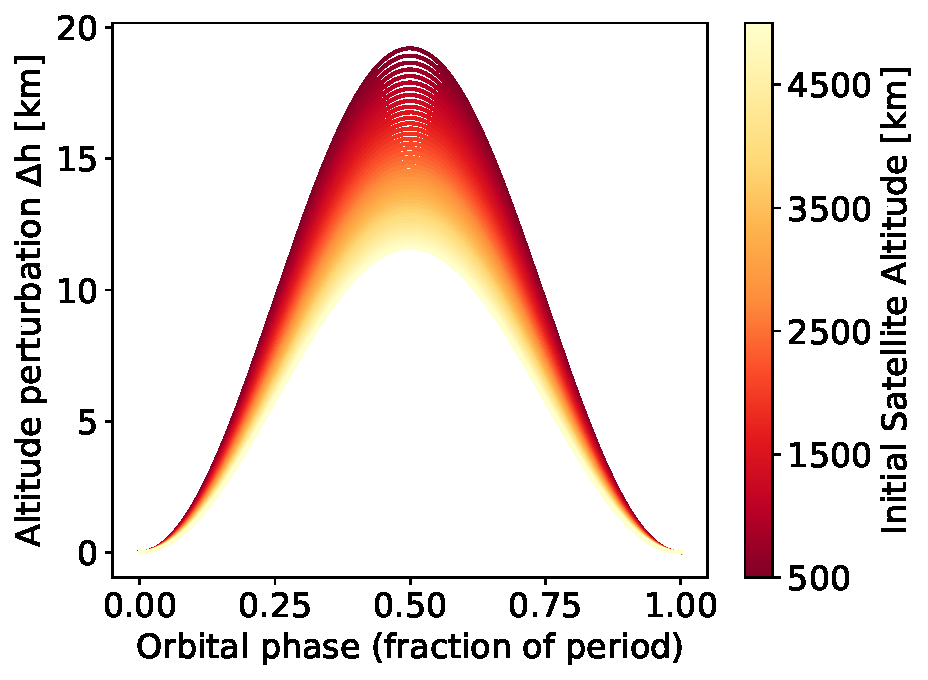
\includegraphics[width=0.4\textwidth]{figures/delta-h.pdf}
    \caption{}
    \label{fig:delta-h}
\end{wrapfigure}

When attempting to track a satellite for long periods of time, the oblateness of the Earth cannot be neglected \cite{bate1971}. The effects of the oblateness of the Earth is quantified in the dimensionless quantity $J_2$, the second zonal harmonic. The Earth, with an oblateness of $3.353 \times 10^{-3}$, has a $J_2$ value of $1.083 \times 10^{-3}$ \cite{curtis2005}. To overcome this, we choose an inclincation of zero for the satellite's orbit and enforce an eccentricty of zero. This allows to keep the \textbf{radius of the Earth fixed} at the value of the equatorial radius, $R_e = 6.378 \times 10^6$ m \cite{luzum2011}. When accounting for perturbations we found that the difference in observables is not worth the computational intensity. For example, one can perform a simulation of a satellite with altitude $h$ both non-perturbed and perturbed and compute the difference $\Delta h = h - h_{\text{per}}$ to arrive at Fig. \ref{fig:delta-h}. Fig. \ref{fig:delta-h} reveals that the perturbations have larger impact for lower altitudes. However, \(\Delta h\) (20 km for an initial altitude of 500 km) is negligible when we recall that we consider radii, $r = R_e + h$, and $R_e \gg \Delta h$.\footnote{One may argue that the inclination and drift may also change as a result of the perturbations. However, since symmetry is preserved about the equatorial plane, the inclination remains unaffected. Also, drift was found to be negligible for singular orbits when generating Fig. \ref{fig:delta-h}.}

\subsubsection{Elementary Dynamics}

In the absence of perturbations, we refer back to classical mechanics to find that the equation of motion for the satellite is
\begin{equation}\label{eq:eom-sat}
    \theta\qty(t) = \theta^0 + \omega_\theta t,
\end{equation}
where $\theta^0$ is the initial angular displacement of the satellite and $\omega_\theta^2 = \mu.r^{-3}$ is the square of the angular velocity.

%   -   -   -   -   -   -   -   -   -   -   -   -   -   -   -   -   -   -   -   -   -   -   -   -   -   -

\subsection{Ground Station Arrangement}

\begin{wrapfigure}[15]{r}{0.35\textwidth}
    \centering
    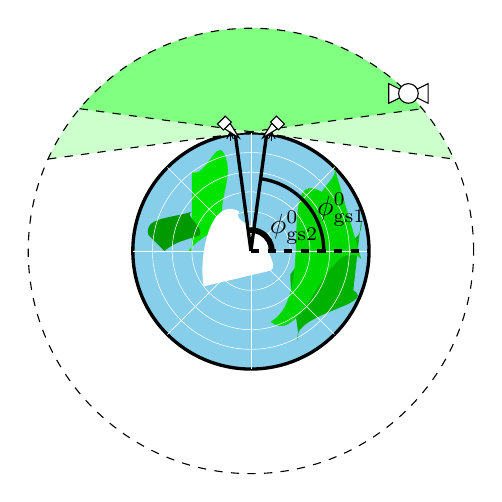
\begin{tikzpicture}[scale=0.5]
        % Earth --  --  --  --  --  --  --  --  --  --  --  --  --  --  --
        % filled blue circle
        \draw[very thick, fill=SkyBlue] (0,0) circle (3cm);
    
        % landmasses
        \fill[green!90!black] (-1.5, 2) to[out=-20, in=120] (-0.7, 2.5) 
            to[out=-60, in=140] (-0.5, 0.5) 
            to[out=100, in=200] (-1.5, 0);
        
        \fill[green!70!black] (2.8, 0.8) to[out=-80, in=60] (1, -0.6) 
            to[out=-90, in=90] (1.2, -2.3) 
            to[out=110, in=-30] (2.6, -1);
    
        \fill[green!60!black] (-2.2, 0) to[out=40, in=200] (-1.3, 0.4) 
            to[out=60, in=-160] (-1.5, 1) 
            to[out=-160, in=110] (-2.6, 0.4);
    
        \fill[green!85!black] (2.8, -0.2) to[out=140, in=-40] (0.5, -1.8) 
            to[out=30, in=150] (1.8, 1.5) 
            to[out=60, in=-60] (2.1, 2.2);

        % Arctic ice cap
        \fill[white] (0.5, -0.5) to[out=30, in=200] (0.5, 0.2) 
            to[out=60, in=-120] (-0.3, 1) 
            to[out=150, in=100] (-1.2, -0.9);
    
        % latitude circles
        \draw[very thin, white] (0,0) circle (2.5cm);
        \draw[very thin, white] (0,0) circle (2cm);
        \draw[very thin, white] (0,0) circle (1.5cm);
        \draw[very thin, white] (0,0) circle (1cm);
    
        % Add meridians
        \foreach \angle in {0, 45, 90, 135, ..., 315}
            \draw[very thin, white] (0,0) -- (\angle:3cm);

        % Vernal equinox
        \draw[very thick, dashed] (0,0) -- (3,0);
        %  --  --  --  --  --  --  --  --  --  --  --  --  --  --  --  -- 

        % Visibility windows  --  --  --  --  --  --  --  --  --  --  --  
        % Shading the region between the circle and the lines
        \begin{scope}
            \clip (0,0) circle (5.65685424949cm);        % Clip to the inside of the circle
            \fill[green!20] (-4.35301, 3.61266) -- (5.15301, 2.33377) -- (2.43207, 8) -- (0.75425,12) -- (-1.22714, 8) -- cycle; % Shade the region bounded by the line and the circle
        \end{scope}
        
        \begin{scope}
            \clip (0,0) circle (5.65685424949cm);
            \fill[green!20] (-5.15301, 2.33377) -- (4.35301, 3.61266) -- (1.28135, 8) -- (-0.75425,12) -- (-2.52982, 8) -- cycle;
        \end{scope}

        \begin{scope}
            \clip (0,0) circle (5.65685424949cm);
            \fill[green!50] (-4.35301, 3.61266) -- (0, 3.02703) -- (4.35301, 3.61266) -- (2.03069,8) -- (0, 12) -- (-2.03069,8) -- cycle;
        \end{scope}

        % Visibility window lines
        \draw[dashed] (-5.15301, 2.33377) -- (4.35301, 3.61266);
        \draw[dashed] (-4.35301, 3.61266) -- (5.15301, 2.33377);
        %  --  --  --  --  --  --  --  --  --  --  --  --  --  --  --  -- 

        % Ground stations --  --  --  --  --  --  --  --  --  --  --  -- 
        % Right Ground Station
        % Position line
        \draw[very thick] (0,0) -- (0.4, 2.973214);

        % Triangle
        \coordinate (t0) at (0.3, 2.873214);
        \coordinate (t1) at (0.67, 3.103214);
        \coordinate (t2) at (0.53, 3.24321);
        \draw[fill=white] (t0) -- (t1) -- (t2) -- cycle;

        % Lens
        \coordinate (r0) at (0.5, 3.27321);
        \coordinate (r1) at (0.7, 3.073214);
        \coordinate (r2) at (0.85, 3.22321);
        \coordinate (r3) at (0.65, 3.42321);
        \draw[fill=white] (r0) -- (r1) -- (r2) -- (r3) -- cycle;

        % Stand
        \draw (0.53, 3.016187) -- (0.53, 2.8);
        \draw (0.53, 3.016187) -- (0.613, 2.850187);
        \draw (0.53, 3.016187) -- (0.447, 2.850187);

        % Labeling angular displacement
        \draw[very thick] (0.5,0)
            arc[start angle=0, end angle=97.6622550228, radius=0.5cm];
        \draw[very thick] (0.56, 0)
            arc[start angle=0, end angle=97.6622550228, radius=0.56cm]
            node at (1.1, 0.6) {$\phi_{\text{gs2}}^0$};

        % Right Ground Station
        % Position line
        \draw[very thick] (0,0) -- (-0.4, 2.973214);

        % Triangle
        \coordinate (t0) at (-0.3, 2.873214);
        \coordinate (t1) at (-0.67, 3.103214);
        \coordinate (t2) at (-0.53, 3.24321);
        \draw[fill=white] (t0) -- (t1) -- (t2) -- cycle;

        % Lens
        \coordinate (r0) at (-0.5, 3.27321);
        \coordinate (r1) at (-0.7, 3.073214);
        \coordinate (r2) at (-0.85, 3.22321);
        \coordinate (r3) at (-0.65, 3.42321);
        \draw[fill=white] (r0) -- (r1) -- (r2) -- (r3) -- cycle;

        % Stand
        \draw (-0.53, 3.016187) -- (-0.53, 2.8);
        \draw (-0.53, 3.016187) -- (-0.613, 2.850187);
        \draw (-0.53, 3.016187) -- (-0.447, 2.850187);

        % Labeling angular displacement
        \draw[very thick] (1.85,0)
            arc[start angle=0, end angle=82.3377449772, radius=1.85cm]
            node at (2.3, 1.05) {$\phi_{\text{gs1}}^0$};
        %  --  --  --  --  --  --  --  --  --  --  --  --  --  --  --  -- 

        % Satellite --  --  --  --  --  --  --  --  --  --  --  --  --  -
        % Orbit
        \draw[dashed] (0,0) circle (5.65685424949cm);

        % Panels
        \coordinate (p0) at (4.5, 4.25);
        \coordinate (p1) at (3.5, 3.75);
        \coordinate (p2) at (3.5, 4.25);
        \coordinate (p3) at (4.5, 3.75);
        \draw[fill=white] (p0) -- (p1) -- (p2) -- (p3) -- cycle;

        % Center Circle
        \draw[fill=white] (4,4) circle (0.25cm);
        %  --  --  --  --  --  --  --  --  --  --  --  --  --  --  --  -- 
    \end{tikzpicture}
    \caption{}
    \label{fig:scheme}
\end{wrapfigure}

When defining a coordinate frame for the Earth it is common practice to define $+\vu{x}$ in the vernal equinox direction and $+\vu{z}$ in the celestial north pole direction \cite{curtis2005}. $+\vu{y}$ is therefore $\frac\pi2$, counterclockwise when looking down at the Earth from the north pole, relative to $+\vu{x}$. We thus take our ground stations to each be $\epsilon$ radians away from $+\vu{y}$: $\phi_{\text{gs1}}^0 = \frac\pi2 - \epsilon$ and $\phi_{\text{gs2}}^0 = \frac\pi2 + \epsilon$.\footnote{By this definition of \(\epsilon\), the orthodromic distance between the ground stations is $d = 2 R_e \epsilon$.} Akin to Eq. (\ref{eq:eom-sat}), the equations of motion for the ground stations are given by \(\phi_{\text{gs}\,i}\qty(t) = \phi_{\text{gs}\,i}^0 + \omega_e t\) where $\omega_e = 7.292 \times 10^{-5}$ rad$.$s$^{-1}$ \cite{luzum2011} is the mean angular velocity of the Earth.



%   -   -   -   -   -   -   -   -   -   -   -   -   -   -   -   -   -   -   -   -   -   -   -   -   -   -

\subsection{Visibility}

Given the equations of motion for the satellite and both ground stations, one can compute the distance between the satellite and ground station $i$ to be
\begin{equation}
    L_i^2 = r^2 + R_e^2 - 2 r R_e \cos(\qty[\theta^0 - \phi^0_{\text{gs}\, i}] + \qty[\omega_\theta - \omega_e] t)
\end{equation}
via the law of cosines. This expression introduces the notion of \textbf{visibility}: when the satellite is able to \textit{see} a ground station and thus able to communicate with it. In order to ensure no visibility exists part the horizon of a ground station, we define communication to be possible only when $L_i^2 \leqslant L_{\text{max}}^2 = r^2 - R_e^2$. We thus define \textbf{simultaneous visibility} as the time when the satellite is able to communicate with both ground stations all at once. An illustration of \colorbox{green!20}{visibility} and \colorbox{green!50}{simultaneous visibility} is shown in Fig. \ref{fig:scheme}, along with an arbitrarily placed satellite. We limit the simulation to having visibility with at least one ground station. Under this restriction, we arrive at the following initial condition for the satellite:
\begin{equation}
    \theta^0 = \pi - \arccos\qty[- \frac1r \qty(R_e \sin(\epsilon) + \cos(\epsilon) \cdot \sqrt{r^{2} - R_e^2})],
\end{equation}
which has the satellite start in gs1's visibility and enter simultaneous visibility as time goes on.

%   -   -   -   -   -   -   -   -   -   -   -   -   -   -   -   -   -   -   -   -   -   -   -   -   -   -

\subsection{Classical Communication}

Qubits and classical information take time to be distributed and processed. We define the processing time to be $\dd{t} \equiv 1 \times 10^{-3}$ s. The amount of time it takes to communcate is therefore distance- and processing-dependent. We define this \textbf{classical communication time} in the following way:
\begin{equation}
    C_c\qty(t_0) = \frac1c L_i\qty(t_0) + 2\dd{t} + \frac1c L_i\qty(t_0 + \frac1c L_i\qty(t_0) + \dd{t}),
\end{equation}
where the first term is the amount of time it takes the initial qubit to received by ground station $i$, the second term is the amount of processing time on both ends, and the last term is the amount of time it takes the ground station to send classical information (success or failure) back up to the satellite.

%   -   -   -   -   -   -   -   -   -   -   -   -   -   -   -   -   -   -   -   -   -   -   -   -   -   -

\subsection{Loss Model}

\begin{wrapfigure}[9]{r}{0.44\textwidth}
    \centering
    \vspace{-.1\baselineskip}
    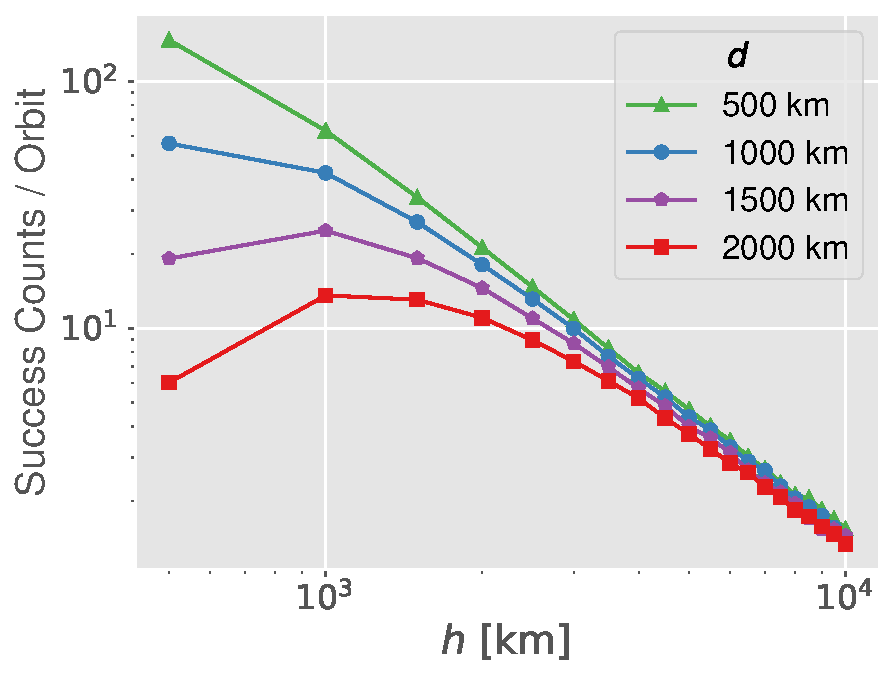
\includegraphics[width=0.44\textwidth]{figures/success-counts.pdf}
    \caption{}
    \label{fig:success-counts}
\end{wrapfigure}

Qubit loss will be the only form of loss that the communication system experiences. This loss will be due to free-space diffraction, as it is main source of loss in space-based quantum networks \cite{khatri2021}. The loss model we consider is the one defined in \cite{khatri2021}\footnote{\cite{khatri2021} is the direct inspiration for this investigation. It's excellent!}. A thorough definition of the loss model is established in the ancilla file, \texttt{ancilla.pdf}. In short, we consider both free space and atmospheric losses. The free space loss occurs due to large distances and device limitations (e.g., beam broadening) while the atmospheric loss is due to interactions with the atmosphere's particles \cite{khatri2021}.


\vspace*{-1.5cm}
\chapter{Results}

We consider satellite altitudes of 500 km up to 10,000 km, incrementing by 500 km. In terms of ground station (gs) separation, \(d\), we consider values from 500 km, roughly the distance from Zacatecas, Zac., MX to Ciudad de M\'{e}xico, to 2,000 km, roughly the distance from Zacatecas, Zac., MX to the Los Angeles, CA. \(d\) is also incremented by 500 km. We implement a Bernoulli process in our simulations and give the satellite a total of 500 orbits for each configuration. The following presentation is that of the averages of our simulation data.

\section{Success Rate}

A success is when the satellite is able to link with both ground stations. Once a success occurs, we store the time at which it occurred as well as the first link age. The satellite then `dumps' the success and attempts to generate another one. Fig. \ref{fig:success-counts} shows the number of successes the satellite is able to achieve per orbit as a function of \(h\) for different values of \(d\). The \textcolor{mygreen}{green} curve shows the trend one would expect: less successes are produced as the satellite altitude increases. The \textcolor{mypurple}{purple} and \textcolor{myred}{red} curves, however, tell a different story. These curves tell us that there exists an optimal value of \(h > \min\qty{h}\) at which the success counts are maxmized. In both cases, this optimal value is \(h = 1,000\) km. Interstingly we also notice that the gs separation becomes irrelevant for large values of \(h\).

\begin{wrapfigure}[19]{r}{0.5\textwidth}
    \centering
    \vspace{-.1\baselineskip}
    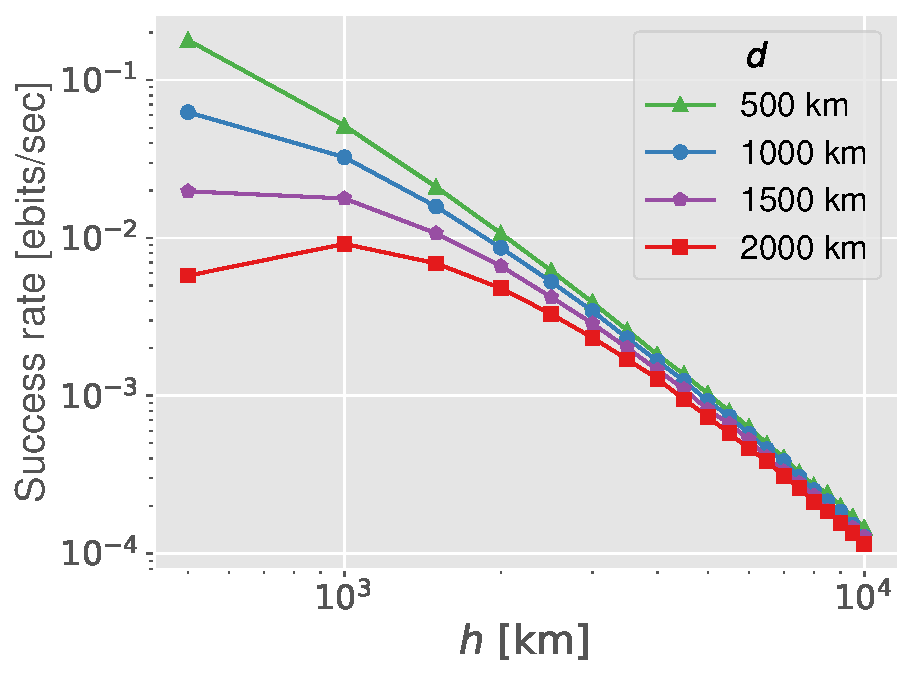
\includegraphics[width=0.5\textwidth]{figures/success-rate.pdf}
    \caption{}
    \label{fig:success-rate}
\end{wrapfigure}

A success rate is shown in Fig. \ref{fig:success-rate}. This rate is computed by the quotient of the number of ebits per orbit (seen in Fig. \ref{fig:success-counts}), divided by the amount of time the satellite spends in visibility:
\begin{equation}
    T_{\text{vis}} = \frac{\theta^f - \theta^0}{\omega_\theta - \omega_e},
\end{equation}
where
\begin{equation*}
    \theta^f \equiv \pi - \theta^0.
\end{equation*}
We divide by this visibility time rather than the period of the orbit since \(T_{\text{vis}} = T_{\text{vis}} \qty(h, d)\) while the the typical period is only a function of \(h\).

We notice that the rates produced in Fig. \ref{fig:success-rate} are much smaller than that in \cite{khatri2021}. This is due to the fact that we have only one ground station our satellite lacks the ability to simultaneously communicate with both gs. Computing the inverse of the data in Fig. \ref{fig:success-rate} thus gives us the expected waiting time for a success. Note, by definition, this is the average amount of time it would take to generate the second link conditioned on the first link already being generated.

\begin{wrapfigure}[14]{l}{0.5\textwidth}
    \centering
    \vspace{-.1\baselineskip}
    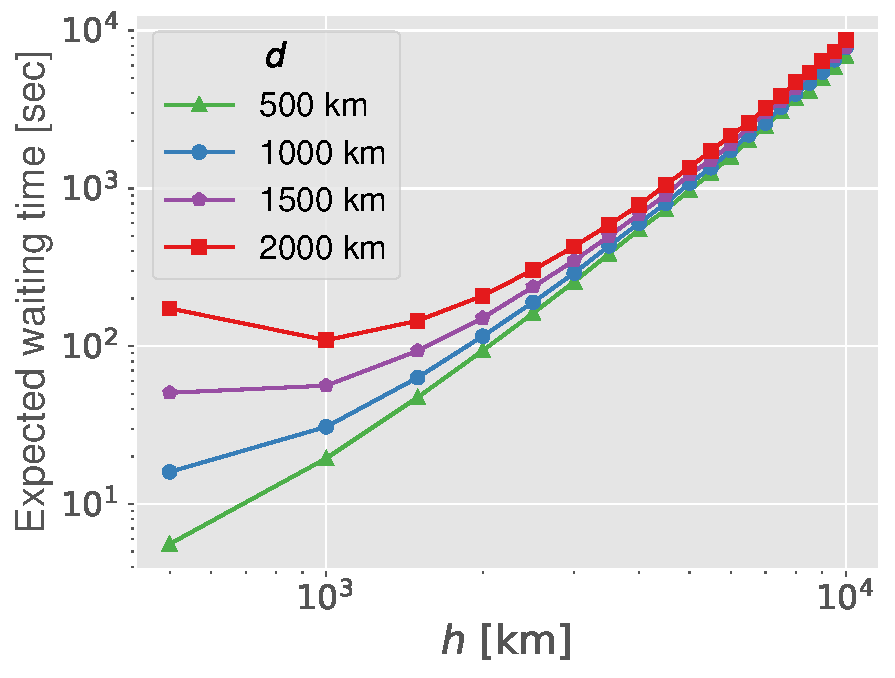
\includegraphics[width=0.5\textwidth]{figures/exp-time.pdf}
    \caption{}
    \label{fig:exp-time}
\end{wrapfigure}

Fig. \ref{fig:exp-time} shows that the minimum expected waiting time is 5.6 sec and occurs for a gs separation of 500 km and a satellite altitude of the same value. The largest expected waiting time occurs for \(h =\) 10,000 km, \(d =\) 2,000 km, with a value of 2.4 hrs. At this same altitude, the smallest value of \(d\) produces an expected waiting time of 1.9 hrs. Keeping these times in mind, in the following section we explore the values that the simulation actually produced.

\section{First Link Age}

Given that the first ground station has succesfully been linked, the first link age is the amount of time it took to generate a succesful link with the second ground station. Since we assume decoherence occurs only on gs memory, this figure of merit is the direct channel to studying how quantum information is affected in a system like the one we are considering.

Fig. \ref{fig:exp-time} told us that satellite altitude is relevant when it comes to expected waiting time, or what we will now call first link age, unlike the behavior we saw in Fig. \ref{fig:success-counts}. The actual data produced by the simulations goes against this and aligns with Fig. \ref{fig:success-counts}. In Fig. \ref{fig:fla}, we see that, starting at \(h =\) 4,000 km (black, dashed line), the first link age is identical for all configurations. We also see, from the \textcolor{myred}{red} and \textcolor{mypurple}{purple} curves in Fig. \ref{fig:fla}, larger values of \(d\) do not necessarily benefit from the smallest value of \(h\). Like in \ref{fig:success-counts}, the best outcome for these curves arrives from a satellite altitude of \(h = 1000\) km. Also, while Fig \ref{fig:exp-time} predicts a minimum first link age of 5.6 sec, Fig \ref{fig:fla} reveals that the actual minimum is 0.42 sec; 7.6\% of the expected value!

\begin{wrapfigure}[16]{r}{0.5\textwidth}
    \centering
    \vspace{-.1\baselineskip}
    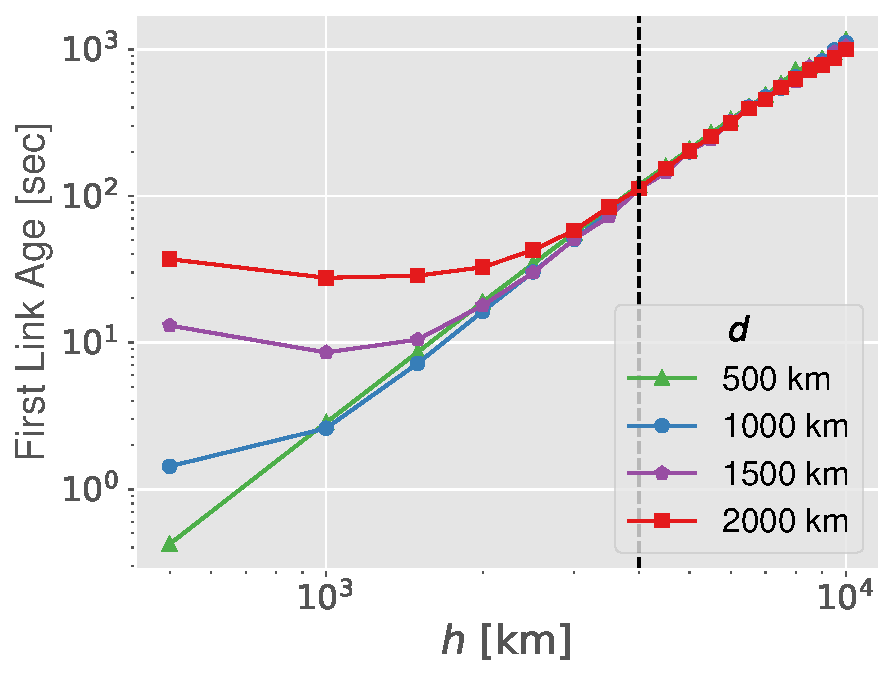
\includegraphics[width=0.5\textwidth]{figures/fla.pdf}
    \caption{}
    \label{fig:fla}
\end{wrapfigure}

Additionally, the largest first age occurs for \(d =\) 500 km\footnote{One would naturally anticipate that the smallest value of \(d\) would always produce the best first link age. However, we've found that for \(h >\) 8,000 km the behavior flips and the smallest first link age is produced by the largest value of \(d\). However, the `best' first link is only \(\sim\)90\% of the worst one in those regions so we don't make a huge point at this difference. Larger values of \(h\) and more values of \(d\) must be considered to confidently establish a trend.} and \(h =\) 10,000 km, with a value of 0.32 hrs. This is 13\% of the value extracted from Fig. \ref{fig:exp-time}.

\section{Quantifying Entanglement}

As a bridge to material we learned in the second half of the class, we take the data in Fig \ref{fig:fla} and see how we can quantify the resulting entanglement between the two gs. We consider two metrics: fidelity and entanglement of formation \cite{wootters1998}. Concretely, we assume the shared Bell state is \(\ket{\Phi^+}\), we apply the single-qubit depolarizing channel to the qubit that is stored on the first gs while the satellite attemps to link with the second one. We assume Markovian \cite{brand2024} noise, where the depolarization rate is \(\gamma = 0.01\) (to counteract the large values we have for the first link age). Under these \textit{super realistic} conditions, we are able to generate Fig. \ref{fig:quant}.

\begin{figure}[h]
    \centering
    \begin{subfigure}[b]{0.4\textwidth}
        \centering
        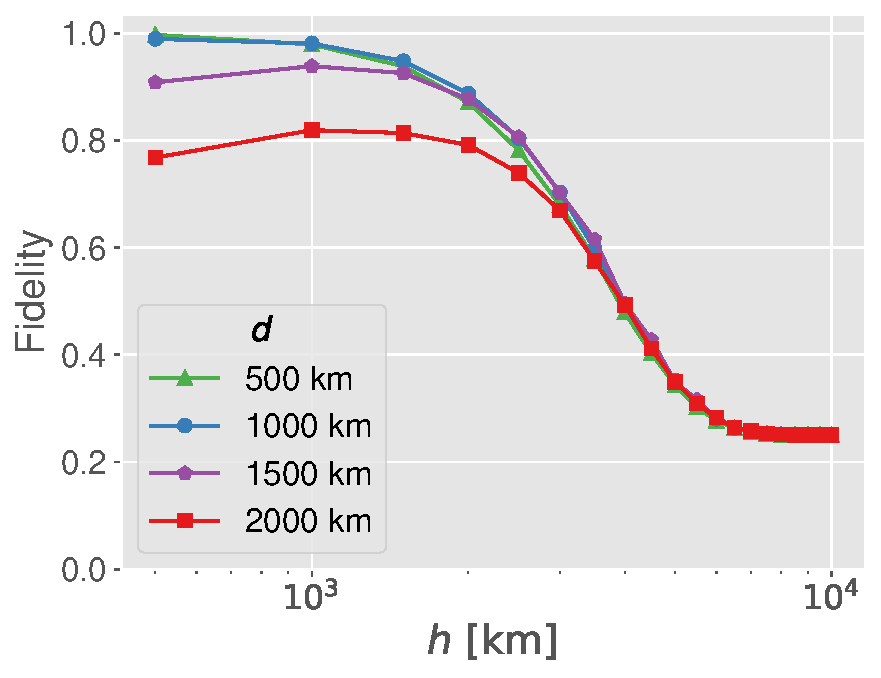
\includegraphics[width=\textwidth]{figures/fidelity.pdf}
        \caption{}
        \label{fig:fid}
    \end{subfigure}
    \hspace{1cm}
    \begin{subfigure}[b]{0.4\textwidth}
        \centering
        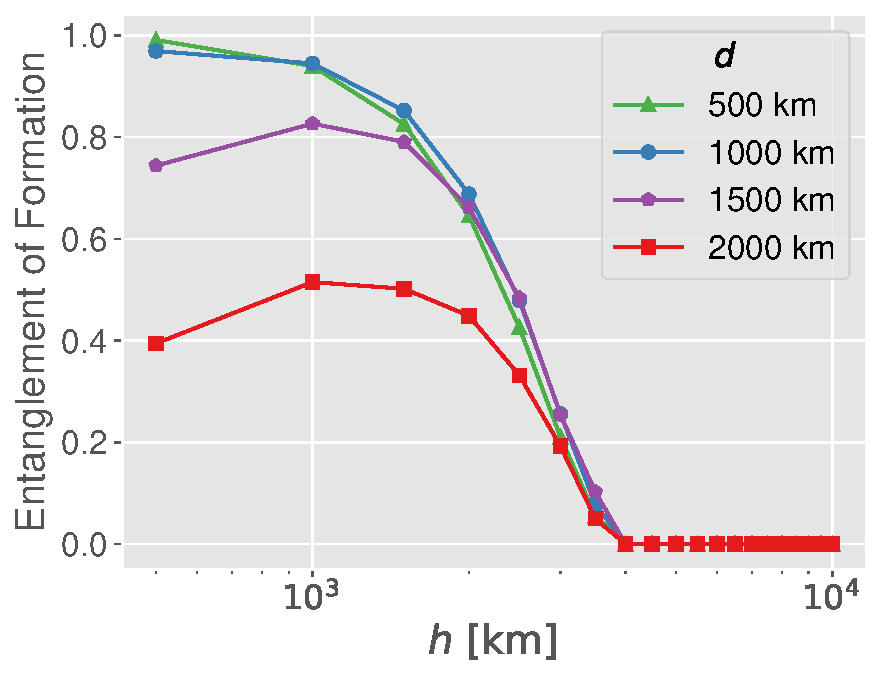
\includegraphics[width=\textwidth]{figures/eof.pdf}
        \caption{}
        \label{fig:eof}
    \end{subfigure}
    \caption{}
    \label{fig:quant}
\end{figure}

\vspace*{-0.5cm}
\section{Conclusions}

My favorite thing I learned in this course is that ``\textbf{fidelity can be a misleading measure of quantum entangled state quality}'' \cite{vardoyan2025}. I have kept it in mind throughout this project and in my own research. The investigation performed here often went against intuition. It is unexpected that the lowest satellite altitude is not always optimal. It is also not expected that a difference in gs spacing of 500 km produces the same fidelity and entanglement of formation, as seen in Fig. \ref{fig:quant}. Fig. \ref{fig:quant} shows similar trend between fidelity and entanglement of formation when it comes to the vairances in \(h\) and \(d\). However, we see that the entanglement of formation values do eventually hit zero while the fidelity never does.

Nevertheless, in this simple experiment we are able to show that satellite communication rates \textit{can} be great, even at an altitude of 500 km. We've skewed the depolariation rate to give us nice-looking figures but further investigation into optimal satellite placement can produce results comparable to what we have here with more realistic values.

\bibliographystyle{apsrev}
\bibliography{bibliography.bib}

\end{document}